\documentclass[11pt]{article}
\usepackage{../cs170}

\def\title{Homework 6}
\def\duedate{10/11/2023, at 10:00 pm (grace period until 11:59pm)}

\begin{document}
\maketitle


Due \textbf{\duedate}

\question{Study Group}
List the names and SIDs of the members in your study group.
If you have no collaborators, you must explicitly write ``none''.

\begin{solution}
	I worked with David He (SID: 3036692442) extensively to come up with a proof of correctness for problem 4,
	and also got a lot of help from the TAs for that problem. Everything else was my own work. 
\end{solution}

\question{Adding Many Edges At Once}

Given an undirected, weighted graph $G(V, E)$, consider the following algorithm to find the minimum spanning tree. This algorithm is similar to Prim's, except rather than growing out a spanning tree from one vertex, it tries to grow out the spanning tree from every vertex at the same time.

\begin{algorithmic}[0]
	\Procedure{FindMST}{$G(V, E)$}
		\State $T \leftarrow \emptyset$
		\While{$T$ is not a spanning tree}
			\State Let $S_1, S_2 \ldots S_k$ be the connected components of the graph with vertices $V$ and edges $T$
			\State For each $i \in \{1, \dots, k\}$, let $e_i$ be the minimum-weight edge with exactly one endpoint in $S_i$
			\State $T \leftarrow T \cup \{e_1, e_2, \ldots e_k\}$
		\EndWhile
		\State \Return $T$
	\EndProcedure
\end{algorithmic}

For example, at the start of the first iteration, every vertex is its own $S_i$.

For simplicity, in the following parts you may assume that no two edges in $G$ have the same weight.

\begin{subparts}
\subpart Show that this algorithm finds a minimum spanning tree.

\begin{solution}
	To show that this algorithm does find an MST, we compare it to the meta algorithm:
	\begin{itemize}
		\item It starts with an empty list, so we're good here
		\item At every iteration, $T$ denotes the part of the MST that we've currently found. Specifically, 
			at every iteration, each $S_i$ is a set that divides the graph into two portions, where 
			there are no edges from $S_i$ to $V \setminus S_i$, so this satisfies this 
			step of the meta algorithm.
		\item To show that the edge adding is correct, the main thing we need to prove that this algorithm doesn't 
			produce a cycle. To do this, consider the following case where a cycle is being created:
			\begin{center}
				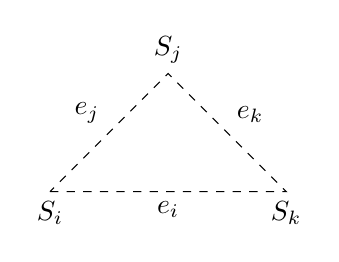
\begin{tikzpicture}
					\draw[dashed] (0, 0) node[below] {$S_i$} -- node[midway, below] {$e_i$} (3, 0) node[below] {$S_k$} -- node[midway, above right] {$e_k$} (1.5, 1.5) node[above] {$S_j$} --  node[midway, above left] {$e_j$} cycle;
				\end{tikzpicture}
			\end{center}
			Here, $S_i, S_j, S_k$ denote connected components, and suppose $S_i$ chose $e_i$ as its 
			minimum weight edge, $S_k$ chose $e_k$ and $S_j$ chose $e_j$. Then, by the definition of the 
			algorithm, we can come up with the following inequalities:
			\begin{align*}
				e_i &< e_j\\
				e_k &< e_i \\
				e_j &< e_k
			\end{align*}
			Combining the first and third equations gives us $e_i < e_k$, but the second equation says that 
			$e_i > e_k$. This is impossible, so we've proven that a cycle cannot be created.

			Then, since the algorithm adds the minimum weight edge between connected components every time, this 
			process of adding edges does indeed satisfy the meta algorithm. 
	\end{itemize}
\end{solution}
\subpart Give a tight upper bound on the worst-case number of iterations of the while loop in one run of the algorithm. Justify your answer. 

\begin{solution}
	The worst case scenario here is when each connected component chooses the same edge, meaning that each 
	of the $k$ connected components ``pair up'' and select an edge that connect each other. After this 
	connection is complete, we have $\frac{k}{2}$ connected components, with $\frac{k}{2}$ edges added. 
	Therefore, in the worst case, at least $\frac{k}{2}$ connected components remain after every iteration. 
	Since we start with $|V|$ connected components (each node forms a single CC), then it takes $\log|V|$ 
	iterations of the while loop. 
\end{solution}
\subpart Using your answer to the previous part, give an upper bound on the runtime of this algorithm. 

\begin{solution}
	Here, the most intensive step is calculating the edge weights that leave each connected component and 
	finding the minimum weight edge for each CC. Since at the beginning we have $|V|$ connected 
	components, then each edge is checked twice, so there are a total of $O(2|E|) = O(|E|)$ checks. 
	Since each check takes constant time, then there's $O(|E|)$ work at every step.
	Therefore in total, there is $O(|E| \log |V|)$ total runtime. 
\end{solution}
\end{subparts}

\pagebreak
\question{Minimum $\infty$-Norm Cut}
In the \textsc{Minimum Infinity-Norm Cut} problem, you are given a connected undirected graph $G=(V, E)$ with positive edge weights $w_e$, and you are asked to find a cut in the graph where the largest edge in the cut is as small as possible (note that there is no notion of source or target; any cut with at least one node on each side is valid). 

Solve this problem in $O(|E|\text{log}|V| + |V| + |E|)$ time. \textbf{Give a 3-part solution.}

\textit{Hint: Minimum Spanning Tree does not require edge weights to be positive.}


\begin{solution}
	As usual, start with a description of the algorithm, then followed by proof of correctness and 
	finally runtime analysis.

	\textbf{Algorithm Description:} Using the hint, we can flip the signs of all
	the edge weights $w_e \to -w_e$, then find an MST on this 
	new graph. Once we've found the MST on this new graph, find the maximum edge weight in this MST. Then, 
	perform a cut on this edge, by outputting the vertices to either side of this edge.  

	\textbf{Proof of Correctness:} By flipping the sign of the edge weights, the largest
	edge weights now become the smallest edge weights, so when we find an MST on the negative graph, this 
	corresponds to finding the maximally spanning tree on the original graph.

	Recall the cut property: Along any given cut, the minimum weight edge in that cut must belong to 
	some MST. Restating this in a more useful way, this is equivalent to saying that any edge selected
	by the MST is the minimum edge in some cut of the graph. In the context of our graph with 
	negative weights, this means that the edges selected by running the MST on the negative graph corresponds 
	to the maximum weight edge in some cut of the original graph. 

	Now, we want to minimize this value, so we want to output the maximum edge weight on the MST, and since 
	this edge weight is negative, this edge corresponds to the minimum weight in the maximally spanning tree.
	Using the cut property, this minimum edge weight in the maximally spanning tree corresponds to the 
	maximum edge weight along some cut of the graph, which is the cut we want to find.

	Finally, since cutting an MST partitions the nodes into two portions, we just want to cut the maximally
	spanning tree along the minimum edge weight we found, which is the maximum edge weight along some cut. 
	Since a cut is represented by a collection of vertices on either side, we can just cut along the maximally 
	spanning tree and output the nodes on either side of it. 
	
	\textbf{Runtime Analysis:} Flipping the edge weights takes $O(|E|)$ time, then running the MST takes 
	(using Kruskal's) takes $O(|V| + |E| \log |V|)$, so in total:
	\[
	O(|E|) + O(|V| + |E| \log |V|) = O(|E| \log |V| + |V| + |E|)
	\] 
	As desired. 
\end{solution}

\pagebreak
\question{Firefighters}

PNPLand is made of $N$ cities that are numbered from $0, 1, \dots N-1$, which are connected by two-way roads. You are given a matrix $D$ such that, for each pair of cities $(a,b)$, $D[a][b]$ is the distance of the shortest path between $a$ and $b$.

We want to pick $K$ distinct cities and build fire stations there. For each city without a fire station, the response time for that city is given by distance to the nearest fire station. We define the response time for a city with a fire station to be 0. Let $R$ be the maximum response time among all cities. We want to create an assignment of fire stations to cities such that $R$ is as small as possible. 

Suppose the optimal assignment of fire stations to cities produces response time $R_{\text{opt}}$. Given positive integers $N,K$ and the 2D matrix $D$ as input, describe an $O(N^2 \cdot K)$ (or faster) greedy algorithm to output an assignment that achieves a response time of $R_g \leq 2 \cdot R_{\text{opt}}$. \textbf{Provide a 3-part solution.} For your proof of correctness, show that your algorithm achieves the desired approximation factor of 2. 

\textit{Hint: $D[a][b]$ represents shortest (metric) distances. So you can use the triangle inequality: $0 \leq D[a][b] \leq D[a][c] + D[c][b]$ for all $a, b, c$}.


\begin{solution}
	We can model this scenario with a graph where the cities are nodes, and the edge weights are the values 
	of $D[a][b]$. 

	\textbf{Algorithm Description:} Start by placing a fire station at an arbitrary node. Then, compute 
	the response time to every other city. Take the edge with the largest response time, and place a fire 
	station there. Then, update the distances to all other cities without fire stations, by comparing whether 
	their distance to the most recently added fire station is shorter than their prior distance. Repeat
	this algorithm until we've run out of fire stations to place. 
	
	\textbf{Proof of Correctness:} Here we need to prove the inequality that $R_g \le 2R_{\text{opt}}$. We 
	will prove this by contradiction, by supposing that $R_g > 2R_{\text{opt}}$. In terms of the optimal 
	solution, this means that no optimal solution on $K$ cities can have a response time of less than $R_g / 2$.

	To prove this, first consider the fire stations that Greedy places. Since the longest 
	response time is $R_g$, then this means that all other fire stations placed by Greedy are at least 
	$R_g$ apart. This is by definition of our Greedy algorithm, which chooses the longest response time 
	at every iteration and places a fire station there, so any response time larger than $R_g$ must already 
	have been resolved by Greedy. Moreover, this means that the response time to any city 
	is at most $R_g$.

	Now consider the optimal solution, which has a response time less than $R_g / 2$. We can think of this 
	response time as a ``radius'' around the cities which extend out $R_g /2$ outward, or a ``diameter'' 
	which extends strictly less than $R_g$ outward.
	Due to this constraint, this 
	means that a single city in the optimal solution cannot service two cities while having their 
	response times both be less than $R_g / 2$, since the distance between each of these cities is at least 
	$R_g$ and we have a diameter of strictly less than $R_g$ on the optimal cities. 

	So, for all the cities where Greedy identified a response time that is larger than $R_g$, our 
	optimal solution cannot hope to cover both cities while still maintaining a radius of less than $R_g/2$. 
	Therefore, $K$ fire stations are still required to guarantee that the maximum response time is $R_g$, and since 
	the optimal solution has $R_{\text{opt}} < R_g / 2$, then this means that the optimal solution must have 
	placed $K+1$ fire stations, which is a contradiction given our original constraint of $K$ cities. Therefore, 
	it cannot be the case that $R_g > 2R_{\text{opt}}$, hence we've proven the approximation factor of 2. 
	
	This solution would not have come to me had it not been for many hours lining up in office hours, so 
	massive credit goes to the TAs along the way who helped me get here.  
	
	\textbf{Runtime Analysis:} At every time step, we have to search the entire array and find the maximum edge 
	weight to add a station to, meaning that there is $O(N^2)$ computation at every step. There are $K$ cities
	where we need to place a fire station, so this process repeats $K$ times. The step where we update 
	the distances has $O(N)$ runtime which is also repeated $K$ times, so in total we have:
	\[
	O(K(N^2 + N)) = O(N^2 \cdot K)
	\] 
	as desired. 

	%\textbf{Proof of Correctness:} Here we need to prove the inequality that $R_g \le 2R_{\text{opt}}$. We will 
	%prove this by contradiction. Suppose that $R_g > 2R_{\text{opt}}$, like in the diagram below:
	%\begin{center}
	%	\begin{tikzpicture}
	%		\draw (0, 0) node[left] {$F_g$} -- node[midway, below] {$R_g > 2R_{\text{opt}}$} (3, 0) node[right] {$C$};
	%	\end{tikzpicture}
	%\end{center}
	%Here, let $F_g$ denote a fire station placed by our greedy algorithm, and $C$ be the ``worst city'' in 
	%terms of response time. Now, we compare this configuration to the optimal solution, of which 
	%there are two possiblities:

	%\textit{Case 1:} This is the situation where in the optimal solution, both cities $F_g$ and $C$ are 
	%serviced by a single fire station $F_o$ in the optimal solution:
	%\begin{center}
	%	\begin{tikzpicture}
	%		\draw (0, 0) node[left] {$F_g$} -- node[midway, below] {$R_g > 2R_{\text{opt}}$} (3, 0) node[right] {$C$};
	%		\draw[red] (0, 0) -- node[midway, above left] {$\le R_{\text{opt}}$} (1.5, 1.5) node[above] {$F_o$} -- node[midway, above right] {$\le R_{\text{opt}}$} (3, 0);
	%	\end{tikzpicture}
	%\end{center}
	%In this case, by the triangle inequality, we have that $R_{\text{opt}} + R_{\text{opt}} \ge R_g > 
	%2R_{\text{opt}}$, which is impossible, so we've arrived at a contradiction. Therefore the statement 
	%$R_g > 2R_{\text{opt}}$ is false, and this case is complete. 

	%\textit{Case 2:} This is the situation where in the optimal solution, $F_g$ and $C$ are serviced by 
	%separate fire stations:
	%\begin{center}
	%	\begin{tikzpicture}
	%		\draw (0, 0) node[left] {$F_g$} -- node[midway, below] {$R_g > 2R_{\text{opt}}$} (3, 0) node[right] {$C$};
	%		\draw[red] (0, 0) -- node[midway, left] {$\le R_{\text{opt}}$} (-0.5, 1.5) node[above] {$F_{o, 1}$};
	%		\draw[red] (3, 0) -- node[midway, right] {$\le R_{\text{opt}}$} (3.5,1.5) node[above] {$F_{o, 2}$};
	%	\end{tikzpicture}
	%\end{center}
	%Here, $F_{o, 1}$ and $F_{o, 2}$ represent the two fire stations that service cities $F_g$ and $C$, with 
	%response time $R \le R_{\text{opt}}$. 

	%In this case, invoking triangle inequality is impossible since we no longer have a triangle. However, notice
	%that since $R_g$ is the maximum service time, then $F_{o, 2}$ could not have been chosen 
	%as a fire station in the greedy algorithm, since had it been chosen then the optimal distance to $C$ would 
	%have been less than or equal to $R_{\text{opt}}$, which is a contradiction since the shortest distance 
	%was assumed to be $R_g > 2R_{\text{opt}}$. 
	%Now, let's draw the connections between $F_{o, 1}$ and $F_{o, 2}$, as 
	%well as $F_g$ to $F_{o, 2}$:
	%\begin{center}
	%	\begin{tikzpicture}
	%		\draw (0, 0) node[left] {$F_g$} -- node[midway, below] {$R_g > 2R_{\text{opt}}$} (3, 0) node[right] {$C$};
	%		\draw[red] (0, 0) -- node[midway, left] {$\le R_{\text{opt}}$} (-0.5, 1.5) node[above] {$F_{o, 1}$};
	%		\draw[red] (3, 0) -- node[midway, right] {$\le R_{\text{opt}}$} (3.5,1.5) node[above] {$F_{o, 2}$};
	%		\draw[red, dashed] (0, 0) -- (3.5, 1.5);
	%		\draw[red, dashed] (-0.5, 1.5) -- (3.5, 1.5);
	%	\end{tikzpicture}
	%\end{center}	
	%Since $R_g$ is the maximum response time among all cities, then we know that the response 
	%time from $F_g$ to $F_{o, 2}$ is at most $R_g$. Further, we know that since $F_{o, 1}$ and $F_{o, 2}$ are 
	%selected in the optimal algorithm, them the distance between those two must be larger than $R_{\text{opt}}$.
	%\footnote{Otherwise, we'd have an edge whose response time is larger than $R_{\text{opt}}$.} Let's mark 
	%these two observations on our diagram:
	%\begin{center}
	%	\begin{tikzpicture}
	%		\draw (0, 0) node[left] {$F_g$} -- node[midway, below] {$R_g > 2R_{\text{opt}}$} (3, 0) node[right] {$C$};
	%		\draw[red] (0, 0) -- node[midway, left] {$\le R_{\text{opt}}$} (-0.5, 1.5) node[above] {$F_{o, 1}$};
	%		\draw[red] (3, 0) -- node[midway, right] {$\le R_{\text{opt}}$} (3.5,1.5) node[above] {$F_{o, 2}$};
	%		\draw[magenta, dashed] (0, 0) -- node[midway, above left] {$\le R_g$} (3.5, 1.5);
	%		\draw[red, dashed] (-0.5, 1.5) -- node[midway, above] {$ > R_{\text{opt}}$} (3.5, 1.5);
	%	\end{tikzpicture}
	%\end{center}	
	%I also changed the color to magenta for clarity. Now, consider the triangle made by $F_g, F_{o, 1}$ and 
	%$F_{o, 2}$. By the triangle inequality, we know that  
	%\[
	%	D[F_g][F_{o, 1}] + D_[F_g][F_{o, 2}] \ge D_[F_{o_1}][F_{o, 2}]
	%\] 
	%This implies that the distance from $F_{o, 1}$ to $F_{o, 2}$ is larger than $R_{\text{opt}} + R_g$! Since 
	%this distance is larger than $R_g$, then this implies that $F_{o, 1}$ and $F_{o, 2}$ actually \textit{do}
	%exist in the greedy solution as their distance is larger than the maximum response time given by Greedy.
\end{solution}
\end{document}

